%% uctest.tex 11/3/94
%% Copyright (C) 1988-2004 Daniel Gildea, BBF, Ethan Munson.
%
% This work may be distributed and/or modified under the
% conditions of the LaTeX Project Public License, either version 1.3
% of this license or (at your option) any later version.
% The latest version of this license is in
%   http://www.latex-project.org/lppl.txt
% and version 1.3 or later is part of all distributions of LaTeX
% version 2003/12/01 or later.
%
% This work has the LPPL maintenance status "maintained".
% 
% The Current Maintainer of this work is Daniel Gildea.
\documentclass[11pt]{ucthesis}
\setlength\parindent{0.5cm}

%% The graphicx package provides the includegraphics command.
\usepackage{graphicx}
\graphicspath{{../../../latex/graphics/}{./figures/}{./graphics/}}
%% The amssymb package provides various useful mathematical symbols
\usepackage{amssymb}
\usepackage{amsmath}
\usepackage{amsthm}
\usepackage{relsize} % \mathlarger
\usepackage{mathtools}
\usepackage{braket}
\usepackage{enumerate, enumitem}
\usepackage{caption}
\usepackage{subcaption}
\usepackage{float}
\usepackage[section]{placeins} % something to do with figures not floating into next section
\usepackage{tikz}
\usetikzlibrary{arrows.meta}

\usepackage{algorithm}
\usepackage[noend]{algpseudocode}
\usepackage{bbm}

\usepackage{etoolbox}
\AtBeginEnvironment{algorithm}{\ssp}
% \AtBeginEnvironment{figure}{\ssp}
\AtBeginEnvironment{equation}{\ssp}
\AtBeginEnvironment{thebibliography}{\ssp}

\makeatletter
\def\BState{\State\hskip-\ALG@thistlm}
\makeatother

\newcommand{\edge}{%
  \mathrel{-}% minus as a relation
  \joinrel\joinrel % some backup
  \mathrel{-}% minus as a relation
}
\newcommand{\notedge}{%
  \mathrel{\mkern2mu}% a small advancement
  \arrownot % a short slash
  \mathrel{\mkern-2mu}% compensate
  \edge
}

\def\dsp{\def\baselinestretch{2.0}\large\normalsize}
\dsp

\newcommand{\vect}[1]{{\it{\boldsymbol{#1}}}}

\begin{document}
% Declarations for Front Matter

\title{Aerial Field Exploration Using The Universal Kriging Method}
\author{Sargis S Yonan}
\degreeyear{2019}
\degreemonth{June}
\degree{MASTER OF SCIENCE}
\chair{Professor Gabriel Hugh Elkaim}
\committeememberone{Professor Numero Dos}
\committeemembertwo{Professor Numero Tres}
\numberofmembers{3} %% (including chair) possible: 3, 4, 5, 6
\deanlineone{Dean Tyrus Miller}
\deanlinetwo{Vice Provost and Dean of Graduate Studies}
\deanlinethree{}
\field{COMPUTER ENGINEERING}
\emphasis{ROBOTICS AND CONTROL}
\campus{Santa Cruz}

\begin{frontmatter}

\maketitle
\copyrightpage

\tableofcontents
\listoffigures
\listoftables

\begin{abstract}
Using an Unmanned Aerial Vehicle (UAV) system, a field of interest can be scanned within a more reasonable time frame compared to conventional scanning techniques involving sattelite and manned-airplane missions. Potentially more nuanced data can be gathered from the UAV made observations because of more desirable fields of view and more customizable sensors on-board.

The Kriging Method, a \textit{Best Linear Unbiased Predictor} (BLUP) commonly used in the field of Geostatistics, exploits the statistical properties of natural phenomena to better predict unobserved points from a set of observed points. Using a modified Universal Kriging Method (for ``on the fly" use ), a prediction and confidence of prediction of the entirety of a given target field can be generated from a set of measurements. From the variances associated with the predictions by the Kriging Method, a corresponding path-planner for UAV field exploration is can be used to reduce the overall uncertainty of field prediction.

A method for the exploration of semi-ergodic fields of interest using aerial observations from UAV using the Kriging Method is introduced. By tessellating a target scan-space into sub-fields with an associated level of prediction confidence, a graph representing the confidence of predictions in adjacent tessellations can be constructed and traversed to reduce the maximum uncertainty of prediction of the entire target space. An experimental simulation and comparisons to other techniques are presented. The method along with the cost-effective nature of a UAV can improve current methods of research, exploration, and natural emergency response. 
\end{abstract}

\begin{dedication}
\null\vfil
{\large
\begin{center}
yerba mate
\vspace{12pt}
\end{center}}
\vfil\null
\end{dedication}


\begin{acknowledgements}
% Mate. Yerba Mate.
%who helped me make sense of the various concepts involved in and out of this project. I would like to extend my thanks to the rest of the Autonomous Systems Lab at UC Santa Cruz for the support and motivation to continue this project everyday.
\end{acknowledgements}

\end{frontmatter}
\chapter{Introduction}
% Why is this problem important? 
% We are introducing the concept of aerial field exploration
Aeriel field exploration is a method in which information from an unknown ground field, a \textit{target field}, can be collected in order to discover traits or track the trends about the field. An exploration method could be a portable generic method for field exploration where a model of the target field phenomena is not known. From a distance above the ground, traits of a target field can be measured using what ever sensor is portable enough to fly or orbit around a field of interest.

%% Here we are going to argue why UAVs are the medium in which we should choose for our explorations
Satellite imagery of Earth has been used for measuring various natural phenomena in the past several decades. Estimating polar ice cap melting rates and exploring the location of an oil spill are among the class of problems solved by this technology. Currently, using a service like the US Forest Services' Moderate Resolution Imaging Spectroradiometer (MODIS) Active Fire Mapping Program, images are updated every 1 to 2 days with a fixed sensor. While this program is helpful for detecting large events with long periods of activity, the sampling rate of this service might not give an emergency response team or a scientist the required resolution and precision in gathered data at their desired rate. The resolution and frequency problem along with the cost associated with building, launching, and maintaining an orbiting Earth satellite might even make some areas of research prohibitive. The use of unmanned aerial vehicles (UAVs) have more recently been used in similar fields of study and in environmental protection. The benefits gained from using UAVs is that of more rapidly acquired data with more easily adjusted accuracy. Furthermore, a UAV can give more nuanced and detailed data on features of a field that are not observable from the distance or field of view of an orbiting satellite. This is because the UAV can be equipped with any compatible sensor and can be deployed from virtually anywhere to fly virtually anywhere. Furthermore, an exploration technique, versus a patrolling or tracking technique, does not require a model of the target field dynamics.

% What have others done before me? How is what I'm doing different? Why is it better?
Presently, scanning fields with unmanned aerial vehicle systems is a task involving flying one or more UAVs in a zig-zag, or other predetermined, maneuver above a target field, while collecting data. This task might take longer than needed to collect the required data, and could potentially ineffectively use the flight time of the UAV which often has a short and limited flight time. Furthermore, scanning every point in a large unknown field is an unrealistic expectation for many UAVs. This is especially a problem if the field as a whole needs is very large and needs to only be explored to a small degree of confidence. A scheme for minimal scanning and effective path planning would be in the benefit of time of the user(s) of the system, and the flown equipment as well. 

% How is what I'm doing different? Why is it better? (part II)
Predictions of the field states must therefore be computed from only a finite set of measurements at known locations. The confidence of predictions should also be attainable through the scheme, as they will be used as metrics to determine the confidence of the predictions. Using a prediction based method to fill in the unseen gaps, though quicker than scanning every point, does not take advantage of the statistical properties of the target field to attempt to minimize flight time and path taken. 

Due to the nature of much of the phenomena one might be interested in scanning in an unknown field, a method that exploits the known stochastic and statistical properties of the field could be used to decrease flight time. A field that exhibits properties of \textit{geospatial autocorrelation}, will be more statistically exploitable to find holes in confidence which can be used to help maneuver the UAV in a direction of low prediction confidence. The Kriging Method, a popular interpolation tool, offers a prediction and a variance of prediction. We can exploit the Kriging variances generated by our prediction to motivate the UAVs to autonomously steer in the areas of least confidence, while traversing over other areas of low prediction confidence, until a minimum confidence in prediction is achieved for an entire unknown target field. The methods introduced attempt to help a user of this system explore an unknown field to a desired level of confidence in a short period of time, using a more methodical path, relative to current exploration techniques. 

\part{Background}

\chapter{Geostatistical Interpolation}
Many of the methods introduced will rely on works developed in the fields of Geostatistics and Geography. Geo-statisticians have developed much of the work surrounding field predictions in the geospatial domain. The Kriging Method, a best linear unbiased predictor, and the heart of the method introduced, produces a prediction based on statistical data gathered from aerial observations, and performs a weighted least-squares using a covariance matrix created from the gathered field data.

Tobler's First Law of Geography \cite{tobler:first_law} states, "Everything is related to everything else, but near things are more related than distant things." Regarding geospatial data, we can say at the very least, there is a positive correlation between observations with a small difference in distance \cite{miller:on_toblers_first_law}. This implies the existence of geospatial autocorrelation in many target fields of interest. This implies a positive correlation between elements in the spatial series that are of interest to the introduced technique. Geospatial autocorrelation is the hypothesis that allows naive prediction techniques, like Inverse Distance Weighting (Section \ref{sec:idw_intro}), to work. 

Furthermore, if the target fields are viewed as an unknown stochastic process, with a generally known underlying Gaussian statistical model, more weight in the Inverse Distance Weighting can be placed on the geospatial elements more related to the point to one desires to predict. A Best Linear Unbiased Predictor (BLUP), like The Kriging Method, does just that. The methods introduced in this chapter are intended to serve as an introduction to the Kriging Method, and aerial geospatial field interpolation in general.

\section{Problem Definitions} \label{sec:defs}
In an effort to be consistent in naming conventions and parameter definitions throughout this work, the problem space will be defined. The conventions will be used throughout the rest of the work.

\subsection{The Field}
The initially unknown field, referred to as the \textit{target field}, will be a square field made up of pixel cells, referred to as \textit{vesicles}, of unit area $a$. The field variable, $Z \in \mathbb{R}^{|Z| \times |Z|}$ therefore has an area of $a|Z|$, where $|Z|$ is the cardinality of the field set $Z$. Each vesicle can also have an associated \textit{age}, or the amount of time elapsed since that cell was last observed, but this parameter will not be used in this work.

\subsection{The Sensor}
For the sake of a simpler introduction to the methods described in this chapter, the basis of the predictions will be observations of interest made using ideal sensors with no measurement noise. The sensors will measure a subset of the area of the entire target field. This area will be referred to as the \textit{sensor footprint}, and will be equal to the size of a single vesicle of the target field, $a$.

For the methods developed, the locations of the sensor measurements must be known. The locations will be represented as Cartesian coordinates on the field $Z$. For an arbitrary observation of the field $Z$, the location of the measurement will be at coordinates $\vect{s} \in \mathbb{R}^2$, and the corresponding sensor measurement would be $Z(\vect{s})$. 

\subsubsection{Real World Sensing Examples}
If a Global Positioning System (GPS) sensor is used to estimate position, a Haversine Transformation would likely be used to convert Earth longitude and latitude to Cartesian coordinates within the target field. If predicting the current location of a wildfire, for example, an infrared sensor would likely be used to measure the values of interest, thermal output of the field in this case.

\subsection{Autocorrelation in a Field}
Positively correlated geospatial autocorrelation in a field implies the existence of a cluster of similar observed values near one another. The opposite is true when the overall geospatial autocorrelation of a field is negative. We can assume, from Tobler's First Law of Geography, that the fields we will measure will contain positive autocorrelation. This degree of geospatial autocorrelation can be measured, and will be discussed in Section \ref{sec:vario} on Variography.

\begin{figure}[ht!]
    \centering
    \begin{subfigure}[t]{0.5\textwidth}
        \centering
        \includegraphics[width=\linewidth]{figures/generated_field.png}
        \captionsetup{skip=0.5\baselineskip,size=footnotesize}
        \caption{A randomly generated geospatially autocorrelated field.}
		\label{fig:gen_field}
    \end{subfigure}%
    ~ 
    \begin{subfigure}[t]{0.5\textwidth}
        \centering
        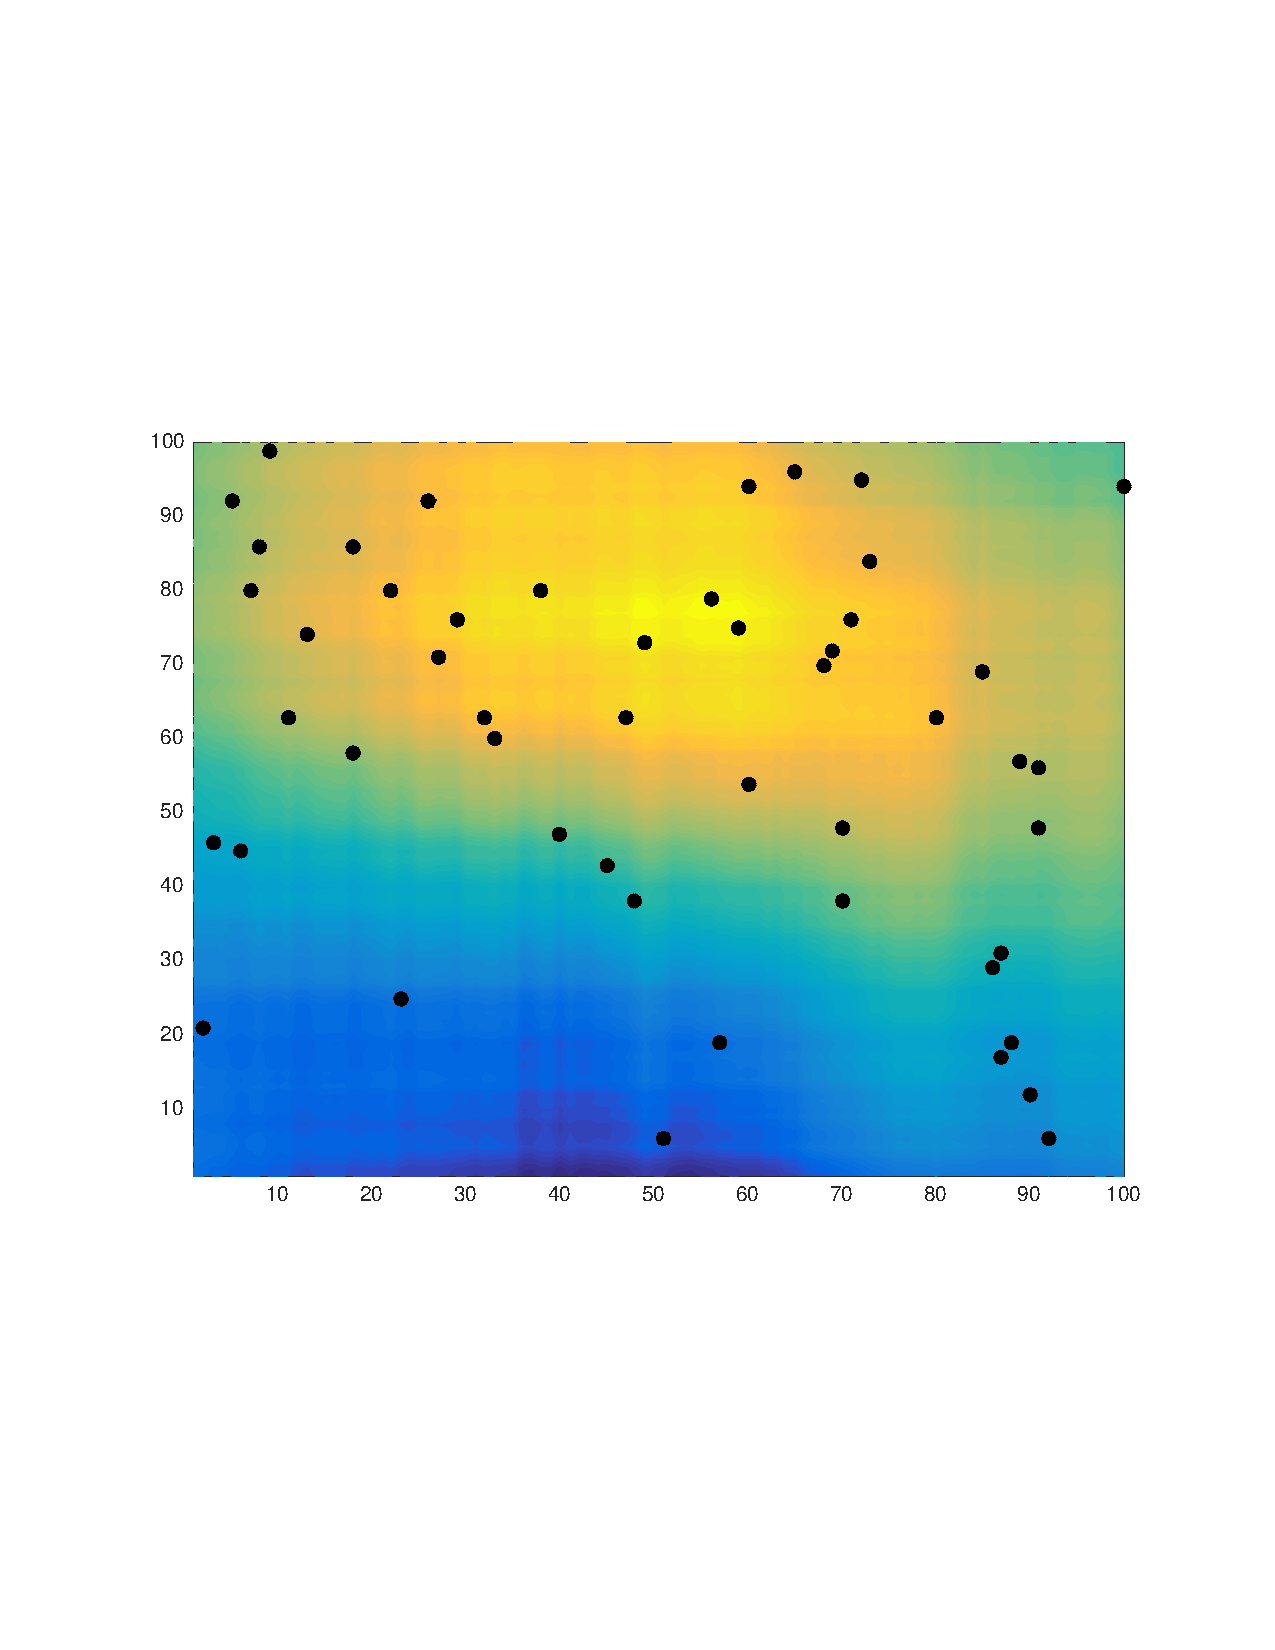
\includegraphics[width=\linewidth]{figures/sampled_generated_field.png}
		\captionsetup{skip=0.5\baselineskip,size=footnotesize}
		\caption{Samples at marked locations were taken of the target field in \ref{fig:gen_field}.}
		\label{fig:sampled_field}
    \end{subfigure}
    \caption{A Gaussian distributed randomly generated spatially autocorrelated field.}
    \label{fig:generated_and_sampled_field}
\end{figure}

\section{Inverse Distance Weighting} \label{sec:idw_intro}
A simple Inverse Distance Weighting (IDW), using Shepard's Method \cite{shepard:idw}, gives a prediction, $\hat{Z}(\vect{s}_j)$, of an unobserved point, $\vect{s}_j$, as a function of the $N \in \mathbb{N}$ observed points, $\{Z(\vect{s}_1), Z(\vect{s}_2), \hdots, Z(\vect{s}_n) \}$.

\begin{equation}
	\hat{Z}(\vect{s}_j)=\begin{cases}
			\dfrac{\sum\limits_{i=1}^N [w(\vect{s}_j, \vect{s}_i)] Z(\vect{s}_i) }{\sum\limits_{i=1}^{N} w(\vect{s}_j, \vect{s}_i)} & \text{if}\ \forall i \mid d(\vect{s}_j,\vect{s}_i) \neq 0\ \\
			Z(\vect{s}_j) & \text{if}\ \exists i \mid d(\vect{s}_j,\vect{s}_i)=0\\
		\end{cases}
\end{equation}
\begin{equation}
	w(\vect{s}_j, \vect{s}_i)=\frac{1}{d(\vect{s}_j,\vect{s}_{i})^{p}}=\|\vect{s}_j-\vect{s}_i\|_{2}^{-p}
\end{equation}

where $p \in \mathbb{R}^{+}$ is the IDW "power parameter". The power parameter, $p$, controls the emphasis on near and far observations on a prediction. As $p$ increases, the predicted values more closely resemble the closest made observation to the prediction location. Inversely, as $p$ gets smaller within $(0, 1]$, more emphasis is drawn from observations made further away.\\

\begin{figure}[ht!]
    \centering
    \includegraphics[width=0.8\linewidth]{figures/idw_predicted_field.png}
    \caption{An inverse distance weighting predicted field generated from the samples taken of Figure \ref{fig:gen_field} at the locations marked in Figure \ref{fig:sampled_field}.}
    \label{fig:idw_field}
\end{figure}

This method can give us a prediction for all possible $\vect{s}_j$ points in a field where a set of observations at known locations were made, as done in Figure \ref{fig:idw_field}. Unfortunately, the method is limited in that it does not take advantage of the underlying stochastic model of the field, $Z$, being observed to make a more methodical weighted sum prediction.

\section{Variography} \label{sec:vario}
Variography is a set of procedures for examining and interpreting spatial dependence and geospatial autocorrelation in observed data. In order to make a more intelligent weighted sum for a prediction, extracting the underlying geospatial autocorrelation function, the \textit{variogram}, of a field will be required. The variogram function will be factored into a classical Inverse Distance Weighting, yielding a Kriging Weighting.

\subsection{The Variogram}
A variogram quantifies dependence for two disjoint observations separated by some distance away. The function therefore yields the covariance between two given points in a stochastic field.

A Variogram is intended to be a continuous function which yields a covariance between two points $Z(\vect{s}_{i})$, $Z(\vect{s}_{j})$, which have not necessarily been observed, but known to be a Euclidean distance $h_{i,j} \in \mathbb{R}$ apart. 

\begin{equation}
h_{i,j} = \| \vect{s}_i - \vect{s}_j \|_2
\end{equation}

Using the assumption made in Equation 2.4.1 of Matherson, 1963 \cite{matheron:geostat}:

\begin{equation}
    Z(\vect{s}_i)=\mu(\vect{s}_i)+\theta(\vect{s}_i)
    \label{eq:matheron:assum}
\end{equation}

Where $\theta(\cdot)$ is a zero-mean intrinsically stationary stochastic process, the Weiner Process. An assumption that the mean $\mu(\cdot) = \bar{Z}$ is only constant in a reasonably small neighborhood of $Z$. This becomes relevant when the sample sizes of the field increase where more reliable means will be derived from local neighborhoods.

It is infeasible to estimate an observation value at each possible point in the field to compute a continuous variogram. A discrete model must first be constructed, and will then be fit into a continuous variogram model. This is done by first constructing a discrete variogram, and then fitting a continuous model to it.

\subsection{The Semi-Variogram}
A Semi-Variogram, or Experimental Variogram, is a discrete function representing the covariance of the observation value difference between two sampled locations that are some distance $h$ apart. By modifying equation 2.4.2, Matheron, 1963 \cite{matheron:geostat} to include an additional boundary to classify a "bin", for two observations $\vect{s}_{i}$ and $\vect{s}_{j}$ in a stochastic field, $Z$, the experimental semi-variogram is defined to be:

\begin{equation} 
    \label{eq:exp_var}
    2\hat{\gamma}(h) := \frac{1}{|N(h,\delta)|}\sum\limits_{\forall \vect{s}_i,\vect{s}_j \in N(h, \delta)}|Z(\vect{s}_i) - Z(\vect{s}_j)|^2 % (Cressie 1993)
\end{equation}

Where $N(h,\delta)$ is the set of all pairs of observed points that are a distance in the interval $[h-\delta, h+\delta]$ away. This distance is referred to as the \textit{lag} between two points. If $\delta = 0$, the semi-variogram is not said to be \textit{binned}.

The experimental variogram conveys the geospatial autocorrelation of a sampled field. As the lag between two given points increases, the covariance also increases. The covariance levels out to a steady value (the \textit{sill}) at some distance in the domain (the \textit{range}). This position in the function marks where the loss of reliable geospatial autocorrelation between two points that are a distance $h$ apart lays.

\subsection{Converting a Semi-Variogram to a Variogram} \label{sec:semitovar}
The intent of fitting a statistical model to an experimental variogram is to approximate the continuous covariance for any two points, that have not necessarily been observed, on $Z$ that are at some known lag apart. It is important to note that a lag larger than the range value is not geospatially autocorrelated \cite{felus:srn}. 

\subsection{Variogram Models}
The continuous variogram will be fit to a statistical model, or \textit{kernel}. The kernel function of the range, $a$, the sill, $s$, and our lag, $h$. Three commonly used models are the following: %P. Goovaerts. Geostatistics for natural resources evaluation. Oxford University Press, New York, 1997.
\subsubsection{The Gaussian Model}

\begin{equation}
	\gamma_g(h, s, a) = s \Bigg[ 1 - \exp \Bigg( -\dfrac{h^2}{a^2} \Bigg) \Bigg]
	\label{eq:gauss_model}
\end{equation}

The Gaussian model will asymptotically reach its sill. The sill would be at the limit as $h$ approaches infinity. The \textit{practical range} is therefore used to refer the point on the domain where the variogram reaches 95\% of its sill.

\subsubsection{The Exponential Model}

\begin{equation}
	\gamma_e(h, s, a) = s \Bigg[ 1 - \exp \Bigg( \dfrac{h}{a} \Bigg) \Bigg]
	\label{eq:exp_model}
\end{equation}

The same rules as the Gaussian model apply to the Exponential model.

\subsubsection{The Spherical Model}

\begin{equation}
	\gamma_s(h, s, a) = \frac{s}{2} \Bigg[ \dfrac{3h}{a} - \Bigg( \dfrac{h}{a} \Bigg)^3 \Bigg]
	\label{eq:sph_model}
\end{equation}

The spherical model will reach an exactly zero slope at the sill and range.

\subsection{Fitting A Semi-Variogram} \label{sec:varfit}

Though there exists no closed-form solution for obtaining a continuous variogram, a nonlinear solver which searches for the minimum error in a cost function of the semi-variogram and the desired kernel would be used.

\begin{equation}
\gamma(h) = \min\ [\gamma_{kernel}(h,s,a) - \hat{\gamma}(h)]^2
\end{equation}

% We specifically will use a modified (we specified bounds to decrease iterations of the function fit) \textit{fminsearch} function in \textit{MATLAB} which is defined to "find the minimum of unconstrained multi-variable function using a derivative-free method". This is done by specifying an objective function to minimize (our desired statistical model) over our experimental semi-variogram.

\begin{figure}[ht!]
    \centering    
	\includegraphics[width=\linewidth]{figures/fit_kernel.png}
	\caption{An experimental variogram generated using Equation \ref{eq:exp_var} from the samples taken in Figure \ref{fig:sampled_field}. $\delta$ was chosen such that for $n$ observations, a total number of $\Big\lfloor \frac{n}{2} \Big\rfloor$ points were plotted. A Gaussian statistical model was fit to the experimental variogram.}
	\label{fig:fit_kernel}
\end{figure}

The \textit{nugget} is defined to be the variance at zero separation, or $\gamma(0)$. This value is exactly zero for ideal measurements, but is generally not for real-life measurements.

\section{The Kriging Method}
The Kriging Method conducts a weighted sum using the continuous variogram model that was fit to the physical observations made. The method can yield a prediction for each vesicle in a target space similar to the Inverse Distance Weighting method described in Section \ref{sec:idw_intro}, but with more statistical robustness.

\subsection{Forms of the Kriging Method}
There exist three major forms of the Kriging Method. All of which differ primarily in the handling of the mean gathered from observations of a target field. The \textit{Simple Kriging Method} makes the assumption that the mean is known and constant throughout the entirety of an observed field. This is of course not the case for fields that are very large as it does not follow Tobler's First Law. The \textit{Ordinary Kriging Method} can deduce the local mean of a neighborhood from a smaller subset of observations in a larger target field. This is done by classifying the larger field into smaller neighborhoods where the mean is only constant within those neighborhoods. Ordinary Kriging has the advantage that the mean is not required to be known before running a prediction. The \textit{Universal Kriging Method} can perform similar local mean calculations as the Ordinary Kriging Method, but does so by fitting a polynomial representing a mean trend model and not from a constant mean value representing that neighborhood \cite{vandergraaf:nnkrig} as seen in Section \ref{sec:varfit} on fitting a variogram.

\subsection{Covariance Matrix From A Variogram} \label{sec:covmat}
From the fit variogram which represents our lag covariances, a \textit{covariance matrix} for $N$ observations, $P \in \mathbb{R}^{N \times N}$, will be constructed. The value of the element $P_{i,j}$, will represent the covariance of the lag between the $i^{th}$ and $j^{th}$ observations. If $i=j$, the value of the element, $P_{i,j}$ would be the variance of that observation. 

\begin{equation}
    P_{i,j} = \text{cov}\{Z(\vect{s}_{i}), Z(\vect{s}_{j})\} = \gamma(\| \vect{s}_i - \vect{s}_j \|_2)
    \label{eq:covvarmatelem}
\end{equation}

\begin{equation}
    P = \begin{bmatrix} 

    \text{var}\{\vect{s}_1\} & \text{cov}\{\vect{s}_1, \vect{s}_2\} & \dots & \text{cov}\{\vect{s}_1, \vect{s}_N\} \\
    
    \text{cov}\{\vect{s}_2, \vect{s}_1\} & \text{var}\{\vect{s}_2\} & \dots & \text{cov}\{\vect{s}_2, \vect{s}_N\} \\

    \vdots & \vdots & \ddots & \vdots  \\
    
    \text{cov}\{\vect{s}_N, \vect{s}_1\} & \text{cov}\{\vect{s}_N, \vect{s}_2\} & \dots & \text{var}\{\vect{s}_N\} \\

    \end{bmatrix}
    \label{eq:covvarmat}
\end{equation}

\subsection{The Proximity Vector}
For any given point on a field, we can construct a \textit{proximity vector}, $\vect{d}_0 \in \mathbb{R}^N$, which contains the covariance of a given point, $\vect{s}_0$ on the field with the $N$ observations made. The $k^{th}$ element of $\vect{d}_N$, would therefore contain the covariance for the lag between point $\vect{s}_0$ and the $k^{th}$ observation made, $\vect{s}_k$.

$$\vect{d}_0(k) = \text{cov}\{Z(\vect{s}_0), Z(\vect{s}_k)\} = \gamma(\| \vect{s}_0 - \vect{s}_k \|_2)$$

\begin{equation}
    \vect{d}_0 = \begin{bmatrix} 
                    \text{cov}\{Z(\vect{s}_0), Z(\vect{s}_1)\} \\
                    \text{cov}\{Z(\vect{s}_0), Z(\vect{s}_2)\} \\
                     \vdots \\
                    \text{cov}\{Z(\vect{s}_0), Z(\vect{s}_N)\} \\
        \end{bmatrix} = 
        \begin{bmatrix} 
                    \gamma(\| \vect{s}_0 - \vect{s}_1 \|_2) \\
                    \gamma(\| \vect{s}_0 - \vect{s}_2 \|_2) \\
                     \vdots \\
                    \gamma(\| \vect{s}_0 - \vect{s}_N \|_2) \\
        \end{bmatrix} 
    \label{eq:proxvect}
\end{equation}

\subsection{The Kriging Weights}
Similarly to the Inverse Distance Weighting method, a set a weights will be computed for each vesicle in the target field. These weights will be referred to as the \textit{Kriging Weights}, or the \textit{error variance vector}. For a given prediction location, $\vect{s}_0$, the Kriging Weight vector, $\vect{\lambda}_0$, will be defined as the product of the inverse of the covariance matrix of the field and the proximity vector of the point to predict.

\begin{equation}
    \vect{\lambda}_{0} = P^{-1}\vect{d}_{0}
    \label{eq:krigweights}
\end{equation}

\subsection{The Kriging Prediction Equation}
The Kriging equation will be used to predict the value, $\hat{Z}(\vect{s}_0)$ of an unobserved location, $\vect{s}_0$. The prediction is a function of the Kriging Weights and a vector of $N$ observations. 

\begin{equation}
    \hat{Z}(\vect{s}_0) = \begin{bmatrix} Z(\vect{s}_1) & Z(\vect{s}_2) & \dots & Z(\vect{s}_N) \end{bmatrix}\vect{\lambda}_{0}
    \label{eq:krigeq}
\end{equation}

\begin{figure}[!]
    \centering
    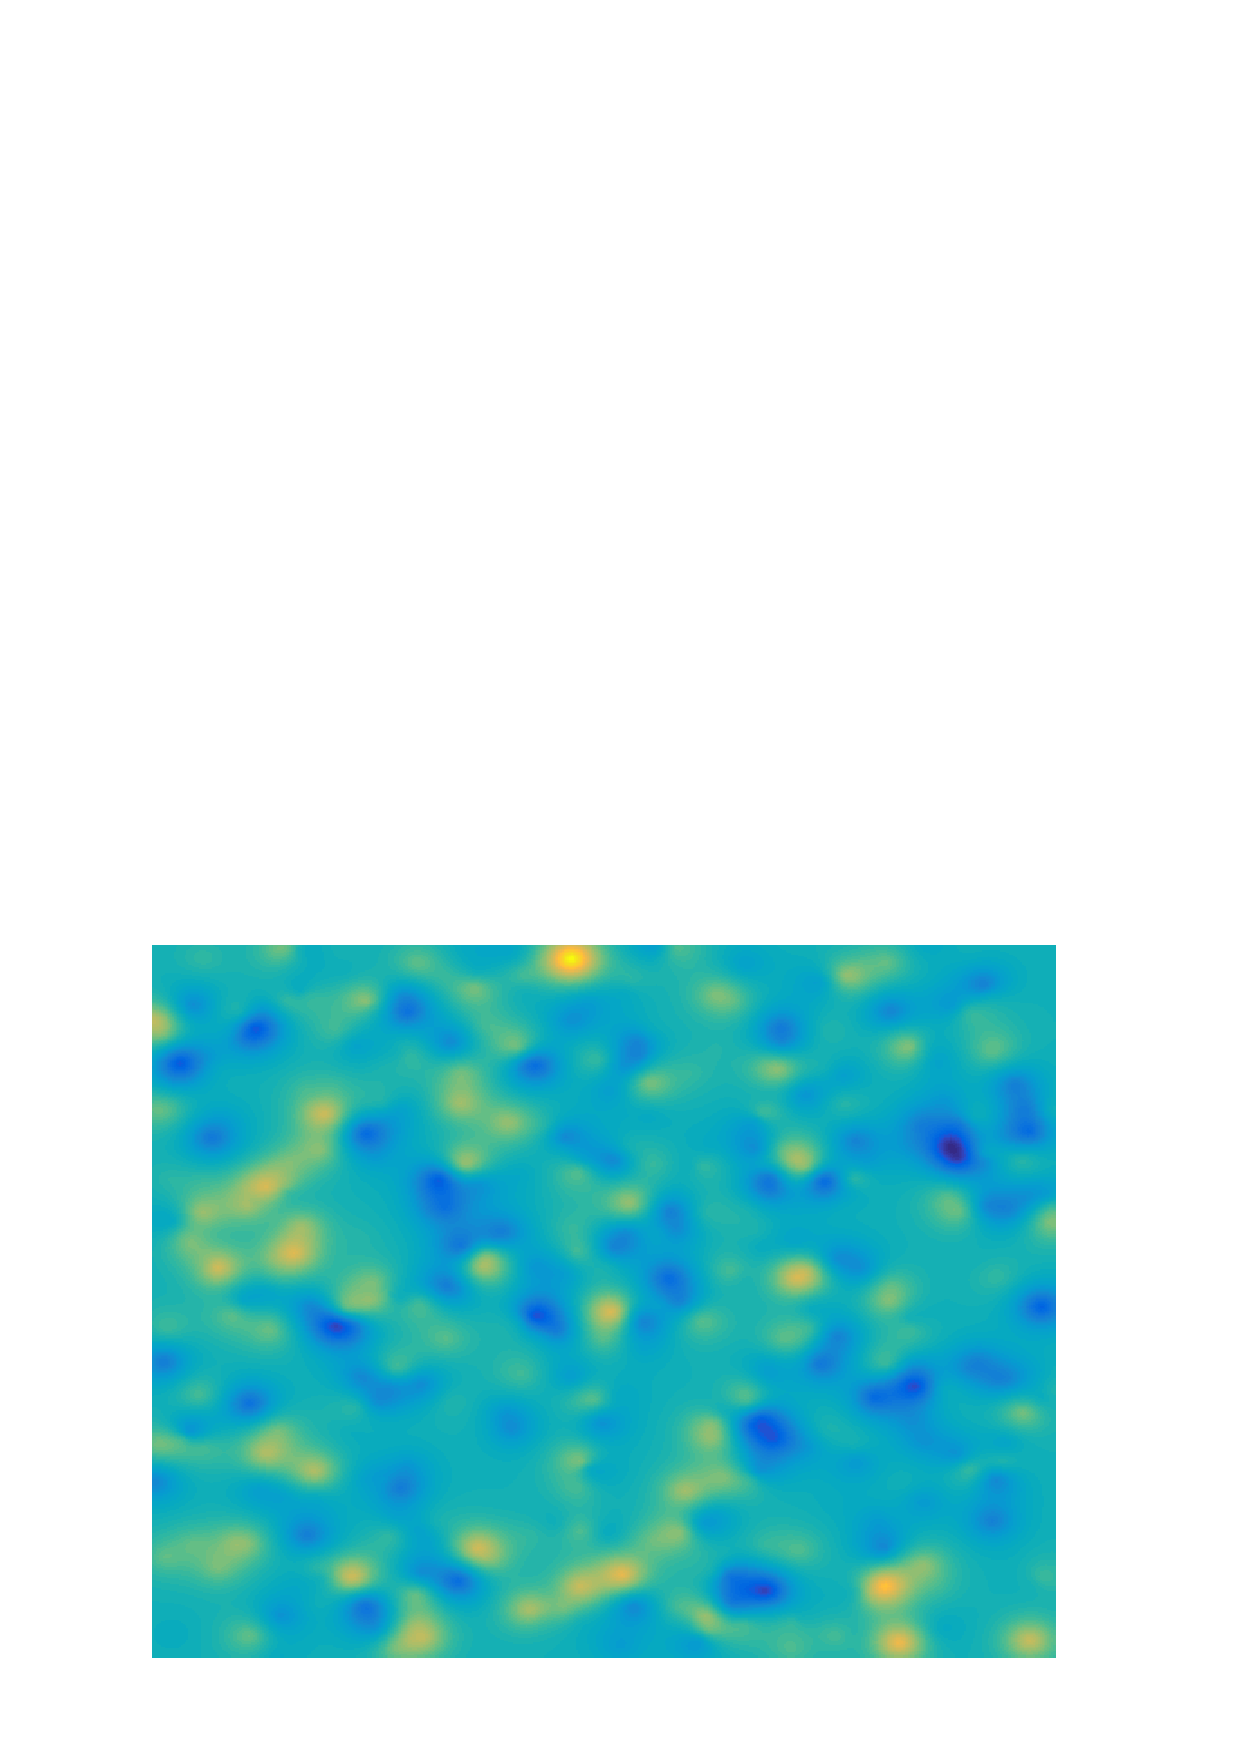
\includegraphics[width=0.8\linewidth]{figures/kriging_prediction.png}
    \caption{A Kriging Method predicted field generated from the samples taken of Figure \ref{fig:gen_field} at the locations marked in Figure \ref{fig:sampled_field}.}
    \label{fig:krig_field}
\end{figure}

\subsection{The Kriging Error}
% look at the wikipedia page
From the method described in Equation \ref{eq:krigeq}, an error can be computed by comparing the predicted value of a previously observed point, $\hat{Z}(\vect{s}_p)$, to the observed value of the point, $Z(\vect{s}_p)$.

\begin{equation}
    \tilde{Z}(\vect{s}_p) = \hat{Z}(\vect{s}_p) - Z(\vect{s}_p) 
    \label{eq:krigerr}
\end{equation}

The Kriging Error value will be used to test the unbiasedness of the predictions made, and is factored into confidence of predictions made.

\subsection{Procedure For Field Prediction Using The Kriging Method}
In order to predict the entirety of a target field from a finite set of $N$ observations and their respective locations, $O$, the Kriging Prediction is run at every possible unobserved vesicle in the target field, $Z$. For a single iteration of collecting observations and making predictions, a covariance matrix must first be constructed, and then a the proximity vector and Kriging Weights are computed for all unobserved vesicles. The Kriging prediction formula is then used to compute the predicted value of each vesicle to predict.

\begin{algorithm}[thpb!]
\caption{Kriging Prediction of Target Field}\label{alg:krig}
\begin{algorithmic}[1]
\Procedure{KrigingPredictField}{$Z$, $O$}
\BState \emph{Generate Semi-Variogram}:
\State $\forall$ $\vect{s}_i$, $Z(\vect{s}_i)$ $\in O$:
\State \ \ \ \ $\hat{\gamma}(h) \gets \vect{s}_i$, $Z(\vect{s}_i)$\\
\BState \emph{Generate Variogram}:
\State $\gamma(h)$ fits to $\hat{\gamma}(h)$\\
\BState \emph{Construct Covariance Matrix}:
\State $\forall (\vect{s}_i,\vect{s}_j) \in O:$
\State \ \ \ \ $h_{i,j} = \|\vect{s}_i - \vect{s}_j\|_2$
\State \ \ \ \ $P_{i,j} = \gamma(h_{i,j})$\\
\BState \emph{Run Kriging Predictions For Target Field}:
\State $\forall$ $\vect{p}_i \in Z$:
\State \ \ \ \ $\vect{d}_{i} = \begin{bmatrix} \gamma(\| \vect{s}_1 - \vec{p}_i \|_2) \dots \gamma(\| \vect{s}_N - \vec{p}_i \|_2) \end{bmatrix}^T$
\State \ \ \ \ $\lambda_{i} = P^{-1}\vect{d}_{i}$
\State \ \ \ \ $\hat{Z}(\vect{p}_i) = \begin{bmatrix} Z(\vect{s}_1) \dots Z(\vect{s}_N) \end{bmatrix} \lambda_{\vec{p}_i}$
\EndProcedure
\end{algorithmic}
\end{algorithm}

When Algorithm \ref{alg:krig} is run on the target field from Figure \ref{fig:generated_field}, for the samples taken in Figure \ref{fig:sampled_field}, a prediction of the entire field can be generated, as seen in Figure \ref{fig:krig_field}.


\section{Limitations of the Kriging Method}
no trends in data\\
its gotta have no obvious clustering \\
assumption of semi/ergodic fields must be used

\chapter{Previous Work}
Oil Spills Boundary Tracking Using Universal Kriging
And Model Predictive Control By UAV - Zhang\\\\
sharon's stuff\\\\
An Efficient Natural Neighbour Interpolation
Algorithm for Geoscientific Modelling - Gold

\part{Procedure For Autonoumous Field Exploration}
\section{Field Exploration Manipulation}
The Variogram represents the confidences of any two predictions that are a distance $h$ apart. We can measure the quality of our predictions, or \textit{confidences} of our predictions, from the fit Variogram. This metric will be used to measure the average uncertainty of state predictions in a subfield, or \textit{neighborhood}, in the target field.

\subsection{Field Tessellation}
By tessellating a target field into natural neighborhoods of Voronoi cells, $\upsilon_i \in \Upsilon$. % talk about this more

\subsection{Neighborhood Prediction Confidence}
A metric for a prediction confidence can be calculated for each neighborhood. A ratio between the average proximity vector and the most ideal proximity vector gives a ratio of confidence of the prediction quality in that neighborhood. % add this to contributions of this paper

% the idea is that we want to fidn the \vec{d}_{max} that gives us the worst \nu_i confidence
\begin{equation}
\label{equ:neigh_conf}
\nu_i = \operatornamewithlimits{argmin}_{\| \vec{d}_{min} \|_2 \in \upsilon_i} \frac{1}{|\upsilon_i|} \large\sum_{i = 1}^{|\upsilon_i|} \frac{\| \vec{d}_{\vec{p}_i} \|_{2}^{-1}} {\| \vec{d}_{min} \|_2^{-1}}
\end{equation}

Where $\vec{p}_i$ is a point in neighborhood $i$, and $|\upsilon_i|$ is the number of points measurable and predictable in neighborhood $i$. The average is normalized to the worst best possible confidence associated with that neighborhood. This is the value associated with the proximity vector with the smallest elements, i.e. least covariance between predicted and measured. % even the measured point in the hood wont be ideal and this will actually give us a decent error still
The best possible prediction confidence occurs when every proximity vector in a given neighborhood is as close as possible to the proximity vector that is composed entirely of elements equal to the smallest value possible in the variogram model. The smallest value of the variogram is referred to as the \textit{nugget} in the Geostatistics literature, and ideally is zero. Due to fields that are not perfectly geospatially autocorrelated and because real-world sensors include some noise, the nugget value is often positive and non-zero. 

\subsection{Total Field Prediction Confidence}
The total field prediction confidence will be defined to be a ration of the function of the neighborhood prediction confidences and sizes to the number of possible points in the field $Z$.

\begin{equation}
\delta = \frac{1}{|Z|} \sum_{i = 1}^{|\Upsilon|} |\upsilon_i| \nu_i
\end{equation}

\subsection{Field Graph Construction}
A graph representing the average confidence of prediction for each neighborhood can be generated. The confidence of a neighborhood, inversely proportional to its uncertainty, will be calculated from a set of proximity vectors from the neighborhood using Equation \ref{equ:neigh_conf}. Neighbors adjacent in the tessellated field are placed in the graph representation as adjacent vertices. For two given vertices in the graph, $\upsilon_i$ and $\upsilon_j$, the corresponding edge weight is the sum of the confidences of the two associated neighborhoods:

\begin{equation}
    w_{ij} = w_{ji} = \nu_i + \nu_j
\end{equation}

\begin{figure}[thpb]
\centering
    \begin{subfigure}[b]{\textwidth}
        \centering
        \includegraphics[width=0.8\textwidth]{./figures/natural_neighborhood_selection.png}
        \captionsetup{skip=0.0\baselineskip,size=footnotesize}
        \caption{Voronoi tessellations of the predicted field in Figure \ref{fig:krig_field}.}
        \label{fig:nat_neigh}
    \end{subfigure}
    \\
    \begin{subfigure}[b]{\textwidth}
        % \includegraphics[width=0.7\textwidth]{./figures/undir_graph_save.png}

        %https://tex.stackexchange.com/questions/270543/draw-a-graph-in-latex-with-tikz
        \centering
        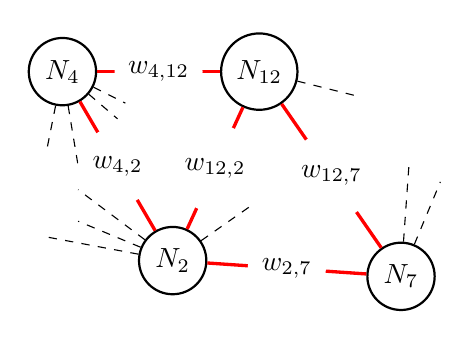
\begin{tikzpicture}
        \begin{scope}[every node/.style={circle,thick,draw}]
            \node (N4) at (0.2,3) {$N_4$};
            \node (N2) at (1.6,.6) {$N_2$};
            \node (N7) at (4.5,.4) {$N_{7}$};
            \node (N12) at (2.7,3) {$N_{12}$};
            
        \end{scope}

        \begin{scope}[>={Stealth[black]},
                      every node/.style={fill=white,circle},
                      every edge/.style={draw=red,very thick}]

            \draw (N7) -- (4.6,1.8) [dashed];
            \draw (N7) -- (5.0,1.6) [dashed];

            \draw (N2) -- (0.4,1.5) [dashed];
            \draw (N2) -- (0.4,1.1) [dashed];
            \draw (N2) -- (0.0,0.9) [dashed];
            \draw (N2) -- (2.6,1.3) [dashed];

            \draw (N4) -- (1.0,2.6) [dashed];
            \draw (N4) -- (0.9,2.4) [dashed];
            \draw (N4) -- (0.4,1.8) [dashed];
            \draw (N4) -- (0,2.0) [dashed];

            \draw (N12) -- (3.9,2.7) [dashed];
            % edge[bend right=90] node
            \path [-] (N4) edge node {$w_{4,2}$} (N2);
            \path [-] (N4) edge node {$w_{4,12}$} (N12);
            \path [-] (N12) edge node {$w_{12,2}$} (N2);
            \path [-] (N12) edge node {$w_{12,7}$} (N7);
            \path [-] (N2) edge node {$w_{2,7}$} (N7);
            

        \end{scope}
        \end{tikzpicture}

        \captionsetup{skip=0.5\baselineskip,size=footnotesize}
        \caption{A subset of the weighted graph representing the adjacencies of the neighbors in Figure \ref{fig:nat_neigh}}
        \label{fig:neigh_graph}
  \end{subfigure}
  \captionsetup{skip=0.5\baselineskip,size=small}
  \caption{The predicted field is tessellated based on the measured point locations in \ref{fig:nat_neigh}. An undirected graph is constructed from the tessellations in \ref{fig:neigh_graph}. The label in each neighborhood identifies the neighborhood name, $\upsilon_i$, and the associated confidence of prediction, $\nu_i$, for that neighborhood.}
\end{figure}

\section{Path Planning}
A path-planning technique based on a shortest-path algorithm is run on the graph. The result will be a path that will guide a UAV into the direction of least confidence while traversing through other uncertain areas. This is because the edge weights are inversely proportional to uncertainty, and maximized in the traversal. 

\subsection{Graph Path Finding}
a*

\subsection{Algorithm For Path Planning}
The path-planning maneuver in turn reduces the uncertainty of prediction of the target field as a whole. 

As more observations are made, the field is re-tessellated and a new graph is created and re-traversed in an attempt to reduce overall uncertainty to a previously specified threshold.

\begin{algorithm}[thpb!]
\caption{Uncertainty Suppressing Field Exploration}\label{alg:uncert}
\begin{algorithmic}[2]
\Procedure{TargetFieldPathPlan}{$Z$}
    \BState \emph{Generate Kriging Prediction}:
    \State $C, \hat{Z} = \textit{KrigingPredictField}(N,Z)$
    \State \textit{Display} $\hat{Z}$\\
    \BState \emph{Tessellate Field}:
    \State $\Upsilon = \textit{Voronoi}(Z, N)$\\
    \BState \emph{Calculate Neighborhood Confidences}:
    \State $\forall \upsilon_i \in \Upsilon$:
    \State \ \ \ \ $\forall \vec{p}_j \in \upsilon_i$:
    \State \ \ \ \ \ \ \ \ $\vec{d}_{\vec{p}_j} = \begin{bmatrix} C_{1,\vec{p}_j} \dots C_{n,\vec{p}_j} \end{bmatrix}^T$
    \State \ \ \ \ $\nu_i = \operatornamewithlimits{argmin}_{\| \vec{d}_{min} \|_2 \in \upsilon_i} \frac{1}{|\upsilon_i|} \large\sum_{i = 1}^{|\upsilon_i|} \frac{\| \vec{d}_{\vec{p}_i} \|_{2}^{-1}} {\| \vec{d}_{min} \|_2^{-1}}$\\
    \BState \emph{Construct Graph Adjacency Matrix, $W$}:
    \State $\forall \upsilon_i \in \Upsilon:$
    \State \ \ \ \ $\forall \upsilon_j \in \Upsilon$:
    \State \ \ \ \ \ \ \ \ \textbf{If} {$\upsilon_j \edge \upsilon{i}$}
    \State \ \ \ \ \ \ \ \ \ \ \ \  $w_{i,j} = w_{j,i} = \nu_{\upsilon_i} + \nu_{\upsilon_j}$
    \State \ \ \ \ \ \ \ \ \textbf{Else}
    \State \ \ \ \ \ \ \ \ \ \ \ \  $w_{i,j} = 0$\\
    \BState \emph{Construct Field Graph}:
    \State $\Gamma = \textit{Graph}(W)$\\
    \BState \emph{Run Path Finding Algorithm on $\Gamma$ To Get a Path $P$}:
    \State $P = \textit{Graph}(W)$\\
    \BState \emph{Explore Field With The Found Path}:
    \State $\forall p_i \in P$:
    \State \ \ \ \ \textit{NavigateTo}($p_i$)\\
    \BState \emph{Calculate Overall Uncertainty}:
    \State $\delta = \frac{1}{|Z|} \sum_{i = 1}^{|\Upsilon|} |\upsilon_i| \nu_i$\\
    \BState{Check Overall Confidence}:
    \State \textbf{If} $\delta < \delta_{max}$:
    \State \ \ \ \ \textbf{goto:} \textit{Generate Kriging Prediction}
    \State \textbf{Else}:
    \State \ \ \ \ \textbf{return}
\EndProcedure
\end{algorithmic}
\end{algorithm}

\part{Other Uses}
% real estate
% crypto price pred.
% gentrify

\part{Simulation Framework}
% \subsection{Flying Engine}
% \subsubsection{Plot Drawing}
% \subsubsection{Way-point Selection}

\chapter{Results}

\chapter{Conclusion}
The potential in a procedure using the Kriging Method as an aerial field exploration technique with UAVs was demonstrated. By characterizing the confidence of the Kriging predictions made from observations in a field, along with a natural neighbor selection technique, a method for path-planning was developed to increase overall confidence in prediction of a target field as a whole. Future work to validate these results with a UAV in the loop will be conducted.

\nocite{*}
\bibliographystyle{plain}
\bibliography{yonan_cmpe_msc_thesis}

\appendix
\chapter{Ancillary Material}

\end{document}
